\documentclass[11pt]{article}
\usepackage[utf8]{inputenc}
\usepackage{amsmath, amssymb, amsthm, geometry, tikz, mathrsfs, mathtools, enumitem}
\usetikzlibrary{arrows.meta, positioning, shapes, calc, decorations.pathreplacing}
\geometry{letterpaper, margin=1in}

% Theorem environments
\newtheorem{theorem}{Theorem}[section]
\newtheorem{lemma}[theorem]{Lemma}
\newtheorem{axiom}{Axiom}
\newtheorem{definition}{Definition}[section]

% Custom commands for problem formatting
\newcommand{\prob}[1]{\vspace{4mm}\noindent\textbf{Problem #1:}}
\newcommand{\sol}{\vspace{2mm}\noindent\textit{Solution: }}
\newcommand{\qedsymbolcustom}{$\blacksquare$}

\title{\textbf{Homework 2: Foundations of Probability and Set Theory}}
\author{Tashfeen Omran}
\date{September 2026}

\begin{document}

\maketitle
\tableofcontents
\newpage

% ==========================================
% PART 1
% ==========================================
\section{Part 1: Comprehensive Introduction, Context, and Prerequisites}

\subsection{Core Concepts \& Axioms}
At its core, probability theory is a measure-theoretic framework used to quantify uncertainty. To transition from intuitive likelihoods to rigorous mathematics, we introduce the concept of a \textbf{Probability Space}, formally defined as a triplet $(\Omega, \mathcal{F}, \mathbb{P})$. 
\begin{itemize}
    \item \textbf{Sample Space ($\Omega$):} The set of all possible distinct, mutually exclusive outcomes of a random experiment. In the discrete case, we often denote this as $S$. Points in $S$ are called \textit{simple events} or \textit{sample points}.
    \item \textbf{Event Space ($\mathcal{F}$):} A collection of subsets of $\Omega$. For finite discrete spaces, this is typically the power set $\mathcal{P}(\Omega)$. Any subset $A \subseteq \Omega$ is called a \textit{compound event}.
    \item \textbf{Probability Measure ($\mathbb{P}$):} A set function mapping events to real numbers, $\mathbb{P}: \mathcal{F} \to [0, 1]$, which dictates the likelihood of an event occurring.
\end{itemize}

\subsection{Intuition and Set-Theoretic Foundations}
Events are evaluated using classical set theory operations. If an experiment is performed and yields outcome $\omega$, we say an event $A$ ``occurred'' if $\omega \in A$. Consequently:
\begin{itemize}
    \item The union $A \cup B$ means ``$A$ occurs \textit{or} $B$ occurs''.
    \item The intersection $A \cap B$ means ``$A$ occurs \textit{and} $B$ occurs''.
    \item Two events are \textit{mutually exclusive} (disjoint) if $A \cap B = \emptyset$.
    \item The complement $\overline{A}$ (or $A^c$) means ``$A$ does \textit{not} occur''.
\end{itemize}

\subsection{Historical Context and Motivation}
Historically, probability began in the 17th century through correspondence between Pierre de Fermat and Blaise Pascal attempting to solve gambling disputes (such as the ``problem of points''). For centuries, it remained a loose collection of combinatorial tricks and intuitive relative frequencies. It wasn't until 1933 that Russian mathematician Andrey Kolmogorov published \textit{Foundations of the Theory of Probability}, resolving foundational crises by rooting probability firmly within the abstract rigidity of Lebesgue's measure theory. This formalized randomness, paving the way for modern statistical inference, quantum mechanics, and stochastic modeling.

\subsection{Key Theorems and Kolmogorov's Axioms}
Any valid probability assignment must satisfy Kolmogorov's Axioms (referred to as Definition 2.6 in the text):
\begin{enumerate}
    \item \textbf{Axiom 1 (Non-negativity):} For any event $A$, $\mathbb{P}(A) \ge 0$.
    \item \textbf{Axiom 2 (Normalization):} $\mathbb{P}(\Omega) = 1$.
    \item \textbf{Axiom 3 (Countable Additivity):} If $A_1, A_2, \dots$ are mutually exclusive events ($A_i \cap A_j = \emptyset$ for $i \neq j$), then $\mathbb{P}\left(\bigcup_{i=1}^\infty A_i\right) = \sum_{i=1}^\infty \mathbb{P}(A_i)$.
\end{enumerate}

\subsection{Prerequisites}
Mastery of this chapter strictly requires:
1. \textbf{Naive Set Theory:} De Morgan's Laws, distributive properties, and subset definitions.
2. \textbf{Combinatorics:} Binomial coefficients ($\binom{n}{k}$) and counting principles.
3. \textbf{Basic Logic:} Understanding logical equivalences ($\iff$) and implications ($\implies$).

% ==========================================
% PART 2
% ==========================================
\section{Part 2: Detailed Homework Solutions}

\prob{2.1}
Let $S = \{FF, FM, MF, MM\}$. Let $A$ denote the subset containing no males, $B$ containing two males, and $C$ containing at least one male. List the elements of $A, B, C, A \cap B, A \cup B, A \cap C, A \cup C, B \cap C, B \cup C,$ and $C \cap B$.

\sol 
Using the definitions provided:
\begin{itemize}
    \item $A = \{FF\}$
    \item $B = \{MM\}$
    \item $C = \{FM, MF, MM\}$
\end{itemize}
We compute the requested set operations:
\begin{align*}
    A \cap B &= \{FF\} \cap \{MM\} = \emptyset \\
    A \cup B &= \{FF, MM\} \\
    A \cap C &= \{FF\} \cap \{FM, MF, MM\} = \emptyset \\
    A \cup C &= \{FF, FM, MF, MM\} = S \\
    B \cap C &= \{MM\} \cap \{FM, MF, MM\} = \{MM\} \\
    B \cup C &= \{MM\} \cup \{FM, MF, MM\} = \{FM, MF, MM\} = C \\
    C \cap B &= B \cap C = \{MM\}
\end{align*}

\prob{2.2}
Suppose $A$ and $B$ are events. Write expressions involving unions, intersections, and complements that describe: (a) Both occur, (b) At least one occurs, (c) Neither occurs, (d) Exactly one occurs.

\sol 
\begin{itemize}
    \item[\textbf{a)}] \textbf{Both occur:} $A \cap B$.
    \item[\textbf{b)}] \textbf{At least one occurs:} $A \cup B$.
    \item[\textbf{c)}] \textbf{Neither occurs:} $\overline{A} \cap \overline{B}$ (which is equivalent to $\overline{A \cup B}$ by De Morgan's Law).
    \item[\textbf{d)}] \textbf{Exactly one occurs:} $(A \cap \overline{B}) \cup (\overline{A} \cap B)$. This represents the symmetric difference $A \Delta B$.
\end{itemize}

\prob{2.3}
Draw Venn diagrams to verify DeMorgan's laws: $\overline{A \cup B} = \overline{A} \cap \overline{B}$ and $\overline{A \cap B} = \overline{A} \cup \overline{B}$.

\sol 
While standard Venn diagram verification consists of shading regions on paper to show graphical equivalence, we provide the rigorous algebraic element-wise proof which forms the basis of the visual truth:
\begin{proof}[Proof (Direct logical equivalence)]
Let $x$ be an arbitrary element in the universal set $S$.
\begin{align*}
    x \in \overline{A \cup B} &\iff x \notin (A \cup B) \\
    &\iff \neg(x \in A \lor x \in B) \quad \text{(Definition of Union)} \\
    &\iff (x \notin A) \land (x \notin B) \quad \text{(Logical De Morgan's Law)} \\
    &\iff (x \in \overline{A}) \land (x \in \overline{B}) \\
    &\iff x \in \overline{A} \cap \overline{B}
\end{align*}
Since both sets contain exactly the same elements, $\overline{A \cup B} = \overline{A} \cap \overline{B}$. The proof for the second law is strictly symmetric, replacing $\lor$ with $\land$.
\end{proof}

\prob{2.4}
If $A$ and $B$ are two sets, draw Venn diagrams to verify:
a) $A = (A \cap B) \cup (A \cap \overline{B})$
b) If $B \subset A$, then $A = B \cup (A \cap \overline{B})$.

\sol
As in 2.3, the graphical equivalent corresponds to this formal logic:
\begin{proof}[Proof for (a)]
By the distributive law of sets:
$ (A \cap B) \cup (A \cap \overline{B}) = A \cap (B \cup \overline{B}) = A \cap S = A $.
\end{proof}
\begin{proof}[Proof for (b)]
If $B \subset A$, then by definition $B \cap A = B$. Substituting this into identity (a):
$A = (A \cap B) \cup (A \cap \overline{B}) \implies A = B \cup (A \cap \overline{B})$.
\end{proof}

\prob{2.5}
Use identities $A = A \cap S$ and $S = B \cup \overline{B}$ and a distributive law to prove algebraically:
a) $A = (A \cap B) \cup (A \cap \overline{B})$.
b) If $B \subset A$ then $A = B \cup (A \cap \overline{B})$.
c) Show that $(A \cap B)$ and $(A \cap \overline{B})$ are mutually exclusive.
d) Show that if $B \subset A$, $B$ and $(A \cap \overline{B})$ are mutually exclusive.

\sol 
\begin{itemize}
    \item[\textbf{a)}] $A = A \cap S = A \cap (B \cup \overline{B})$. By the distributive law of intersection over union, $A = (A \cap B) \cup (A \cap \overline{B})$.
    \item[\textbf{b)}] Given $B \subset A$, any element $x \in B$ implies $x \in A$. Therefore, the intersection $A \cap B = B$. Substituting this into the result from (a) gives $A = B \cup (A \cap \overline{B})$.
    \item[\textbf{c)}] Two sets are mutually exclusive if their intersection is the empty set $\emptyset$.
    \[ (A \cap B) \cap (A \cap \overline{B}) = A \cap A \cap (B \cap \overline{B}) = A \cap \emptyset = \emptyset \]
    \item[\textbf{d)}] Given $B \subset A$, $B \cap (A \cap \overline{B}) = (B \cap A) \cap \overline{B} = B \cap \overline{B} = \emptyset$. Thus they are mutually exclusive.
\end{itemize}

\prob{2.6}
From a survey of 60 students: 9 live off campus, 36 are undergrads, 3 are undergrads living off campus. Find the number of students who were:
a) undergrads, living off campus, or both.
b) undergrads living on campus.
c) graduate students living on campus.

\sol 
Let $S$ be the set of all students ($|S|=60$), $U$ be undergraduates ($|U|=36$), $O$ be off-campus ($|O|=9$). We are given $|U \cap O| = 3$.
\begin{itemize}
    \item[\textbf{a)}] By the Principle of Inclusion-Exclusion:
    $ |U \cup O| = |U| + |O| - |U \cap O| = 36 + 9 - 3 = 42 $
    \item[\textbf{b)}] On campus means $\overline{O}$. We seek $|U \cap \overline{O}|$:
    $ |U \cap \overline{O}| = |U| - |U \cap O| = 36 - 3 = 33 $
    \item[\textbf{c)}] Graduate students on campus corresponds to $\overline{U} \cap \overline{O}$:
    By De Morgan's Law, $\overline{U} \cap \overline{O} = \overline{U \cup O}$. 
    $ |\overline{U \cup O}| = |S| - |U \cup O| = 60 - 42 = 18 $.
\end{itemize}

\prob{2.7}
A group of five applicants consists of three men ($M_1, M_2, M_3$) and two women ($W_1, W_2$). Select two. $A$ = no men, $B$ = at least one man. List outcomes in $A, B, A \cup B, A \cap B$.

\sol 
The sample space $S$ consists of all $\binom{5}{2} = 10$ pairs.
$A = \{W_1 W_2\}$. 
$B$ contains all pairs with at least one man. Since $B = \overline{A}$, $B = S \setminus \{W_1 W_2\}$. Thus,
$B = \{M_1 M_2, M_1 M_3, M_1 W_1, M_1 W_2, M_2 M_3, M_2 W_1, M_2 W_2, M_3 W_1, M_3 W_2\}$.
\begin{align*}
    A \cup B &= S \quad \text{(since } B = \overline{A} \text{)} \\
    A \cap B &= \emptyset \quad \text{(since they are mutually exclusive)}
\end{align*}

\prob{2.8}
Two dice are tossed. Let $S = \{(i, j) \mid 1 \le i,j \le 6\}$. 
A: second die is even. B: sum is even. C: at least one is odd. List points in $A, C, A \cap B, A \cap \overline{B}, \overline{A} \cup B, \overline{A} \cap C$.

\sol 
Using formal set-builder notation to avoid exhaustive trivial listing:
\begin{itemize}
    \item $A = \{(i, j) \in S \mid j \in \{2, 4, 6\}\}$. ($|A| = 6 \times 3 = 18$ points)
    \item $B = \{(i, j) \in S \mid (i \text{ even} \land j \text{ even}) \lor (i \text{ odd} \land j \text{ odd})\}$.
    \item $C = \{(i, j) \in S \mid i \text{ is odd} \lor j \text{ is odd}\}$. ($C = \overline{\{(i,j) \mid i,j \text{ both even}\}}$, $|C|=27$)
    \item $A \cap B = \{(i, j) \in S \mid i \in \{2, 4, 6\} \land j \in \{2, 4, 6\}\}$. ($|A \cap B| = 9$)
    \item $A \cap \overline{B} = \{(i, j) \in S \mid i \in \{1, 3, 5\} \land j \in \{2, 4, 6\}\}$. ($|A \cap \overline{B}| = 9$)
    \item $\overline{A} \cup B = \{(i, j) \in S \mid j \in \{1, 3, 5\}\} \cup B$. Since $B$ contains all (even, even) pairs and (odd, odd) pairs, and $\overline{A}$ contains all pairs ending in an odd number (which includes (even, odd) and (odd, odd)), their union is the entire set $S$ minus (odd, even) pairs. So $\overline{A} \cup B = \{(i, j) \in S \mid \neg(i \text{ is odd} \land j \text{ is even})\}$.
    \item $\overline{A} \cap C$: $\overline{A}$ requires $j$ to be odd. If $j$ is odd, the condition for $C$ (at least one is odd) is trivially satisfied. Thus, $\overline{A} \cap C = \overline{A} = \{(i, j) \in S \mid j \in \{1, 3, 5\}\}$.
\end{itemize}

\prob{2.9}
Blood types are A, B, AB, O. Rh factors are + or -. List the sample space.

\sol
$S = \{A+, A-, B+, B-, AB+, AB-, O+, O-\}$.

\prob{2.10}
Proportions of blood phenotypes: A (.41), B (.10), AB (.04), O (.45).
a) List sample space. b) Assign probabilities. c) Find probability of type A or AB.

\sol 
a) $S = \{A, B, AB, O\}$.
b) $\mathbb{P}(A)=0.41$, $\mathbb{P}(B)=0.10$, $\mathbb{P}(AB)=0.04$, $\mathbb{P}(O)=0.45$.
c) Since the events are mutually exclusive simple events: $\mathbb{P}(A \cup AB) = \mathbb{P}(A) + \mathbb{P}(AB) = 0.41 + 0.04 = 0.45$.

\prob{2.11}
$S = \{E_1, E_2, E_3, E_4, E_5\}$. 
a) If $\mathbb{P}(E_1) = \mathbb{P}(E_2) = 0.15, \mathbb{P}(E_3) = 0.4$, and $\mathbb{P}(E_4) = 2\mathbb{P}(E_5)$, find $\mathbb{P}(E_4)$ and $\mathbb{P}(E_5)$.
b) If $\mathbb{P}(E_1) = 3\mathbb{P}(E_2) = 0.3$, find probabilities of the remaining simple events if they are equally probable.

\sol 
By Axiom 2 and 3, $\sum_{i=1}^5 \mathbb{P}(E_i) = 1$.
\textbf{a)} $0.15 + 0.15 + 0.4 + 2\mathbb{P}(E_5) + \mathbb{P}(E_5) = 1 \implies 0.7 + 3\mathbb{P}(E_5) = 1 \implies 3\mathbb{P}(E_5) = 0.3$. 
Thus, $\mathbb{P}(E_5) = 0.1$ and $\mathbb{P}(E_4) = 0.2$.
\textbf{b)} $\mathbb{P}(E_1) = 0.3$ and $3\mathbb{P}(E_2) = 0.3 \implies \mathbb{P}(E_2) = 0.1$.
Let $\mathbb{P}(E_3) = \mathbb{P}(E_4) = \mathbb{P}(E_5) = p$.
$0.3 + 0.1 + 3p = 1 \implies 3p = 0.6 \implies p = 0.2$. 
Thus $\mathbb{P}(E_3) = \mathbb{P}(E_4) = \mathbb{P}(E_5) = 0.2$.

\prob{2.12}
Vehicle arriving at an intersection can turn left (L), right (R), or go straight (S). 
a) List sample space. b) If equally likely, find probability it turns.

\sol 
a) $S = \{L, R, S\}$.
b) Equiprobability implies $\mathbb{P}(L) = \mathbb{P}(R) = \mathbb{P}(S) = 1/3$. The event ``vehicle turns'' is $A = \{L, R\}$. 
$\mathbb{P}(A) = \mathbb{P}(L) + \mathbb{P}(R) = 2/3$.

\prob{2.13}
Alien cover-up opinions: Very likely (VL) .24, Somewhat likely (SL) .24, Unlikely (U) .40, Other (O) .12.
a) What are the simple events? b) Are they equally likely? c) Probability person finds it at least somewhat likely?

\sol 
a) $S = \{VL, SL, U, O\}$.
b) No, they are not equally likely since their explicit empirical probability measures differ (e.g., $0.24 \neq 0.40$).
c) ``At least somewhat likely'' corresponds to $A = \{VL, SL\}$.
$\mathbb{P}(A) = \mathbb{P}(VL) + \mathbb{P}(SL) = 0.24 + 0.24 = 0.48$.

\prob{2.14}
Table of reading glasses: 
Needs glasses (Yes, No) as rows. Uses glasses (Yes, No) as columns.
Data given as probabilities: $P(N_Y, U_Y) = 0.44$, $P(N_Y, U_N) = 0.14$, $P(N_N, U_Y) = 0.02$, $P(N_N, U_N) = 0.40$. Find:
a) Needs glasses. b) Needs glasses but does not use them. c) Uses glasses whether needed or not.

\sol 
Let $N_Y, N_N$ be needing glasses or not. Let $U_Y, U_N$ be using them or not.
a) $\mathbb{P}(N_Y) = \mathbb{P}(N_Y \cap U_Y) + \mathbb{P}(N_Y \cap U_N) = 0.44 + 0.14 = 0.58$.
b) $\mathbb{P}(N_Y \cap U_N) = 0.14$.
c) $\mathbb{P}(U_Y) = \mathbb{P}(N_Y \cap U_Y) + \mathbb{P}(N_N \cap U_Y) = 0.44 + 0.02 = 0.46$.

\prob{2.15}
Oil prospecting: $E_1$ (Hit, Hit)=0.01, $E_2$ (Hit, Miss)=?, $E_3$ (Miss, Hit)=0.09, $E_4$ (Miss, Miss)=0.81. Firm hits on 10\% of its drillings. Find probability:
a) hit on first, miss on second. b) at least one hit.

\sol 
The sum of all simple events must be 1 (Axiom 2):
$0.01 + \mathbb{P}(E_2) + 0.09 + 0.81 = 1 \implies \mathbb{P}(E_2) = 0.09$.
(Note: The premise ``hits on 10\% of its drillings'' is perfectly consistent, as the marginal probability of a hit on the first drilling is $0.01 + 0.09 = 0.10$, and on the second is $0.01 + 0.09 = 0.10$).
a) Hit on first, miss on second corresponds precisely to event $E_2$. Thus, probability is $0.09$.
b) At least one hit is the complement of no hits ($E_4$). 
$\mathbb{P}(\overline{E_4}) = 1 - \mathbb{P}(E_4) = 1 - 0.81 = 0.19$.

\prob{2.16}
Volunteers blood types: 1 in 3 have O+, 1 in 15 have O-, 1 in 3 have A+, 1 in 16 have A-. Find probability selected person has: a) O+ b) O c) A d) neither A nor O.

\sol 
Let the probabilities be defined directly by the proportions:
a) $\mathbb{P}(O+) = 1/3$.
b) Type O implies $O+$ or $O-$. $\mathbb{P}(O) = \mathbb{P}(O+) + \mathbb{P}(O-) = 1/3 + 1/15 = 6/15 = 2/5$.
c) Type A implies $A+$ or $A-$. $\mathbb{P}(A) = \mathbb{P}(A+) + \mathbb{P}(A-) = 1/3 + 1/16 = 19/48$.
d) Neither A nor O corresponds to $\overline{A \cup O}$. By De Morgan's and Axiom 2:
$\mathbb{P}(\overline{A \cup O}) = 1 - (\mathbb{P}(A) + \mathbb{P}(O)) = 1 - \left( \frac{19}{48} + \frac{2}{5} \right) = 1 - \frac{95 + 96}{240} = 1 - \frac{191}{240} = \frac{49}{240}$.

\prob{2.17}
Aircraft defects: 8\% have shaft defects ($S$), 6\% have bushing defects ($B$), 2\% have both ($S \cap B$). Find probability: a) bushing defect? b) shaft or bushing? c) exactly one? d) neither?

\sol 
Given $\mathbb{P}(S)=0.08, \mathbb{P}(B)=0.06, \mathbb{P}(S \cap B)=0.02$.
a) $\mathbb{P}(B) = 0.06$.
b) By the General Addition Rule: $\mathbb{P}(S \cup B) = \mathbb{P}(S) + \mathbb{P}(B) - \mathbb{P}(S \cap B) = 0.08 + 0.06 - 0.02 = 0.12$.
c) Exactly one is $\mathbb{P}(S \cup B) - \mathbb{P}(S \cap B) = 0.12 - 0.02 = 0.10$.
d) Neither is $\mathbb{P}(\overline{S \cup B}) = 1 - \mathbb{P}(S \cup B) = 1 - 0.12 = 0.88$.

\prob{2.18}
Two balanced coins tossed. a) List sample space. b) Assign reasonable probabilities. c) Let A = exactly one head, B = at least one head. List points. d) Find $\mathbb{P}(A), \mathbb{P}(B), \mathbb{P}(A \cap B), \mathbb{P}(A \cup B), \mathbb{P}(\overline{A} \cup B)$.

\sol 
a) $S = \{HH, HT, TH, TT\}$.
b) Assuming independent fair coins, events are equiprobable: $\mathbb{P}(\omega) = 1/4$ for all $\omega \in S$.
c) $A = \{HT, TH\}$, $B = \{HH, HT, TH\}$.
d) By counting sample points:
$\mathbb{P}(A) = 2/4 = 1/2$.
$\mathbb{P}(B) = 3/4$.
$\mathbb{P}(A \cap B) = \mathbb{P}(\{HT, TH\}) = 2/4 = 1/2$.
$\mathbb{P}(A \cup B) = \mathbb{P}(\{HH, HT, TH\}) = 3/4$.
$\overline{A} = \{HH, TT\}$, so $\overline{A} \cup B = \{HH, TT\} \cup \{HH, HT, TH\} = \{HH, HT, TH, TT\} = S$. Thus, $\mathbb{P}(\overline{A} \cup B) = \mathbb{P}(S) = 1$.

\prob{2.19}
Paper supplies from 3 vendors ($V_1, V_2, V_3$) over two days.
a) List sample space. b) Assign probabilities. c) A = same vendor both days, B = $V_2$ at least once. Find $\mathbb{P}(A), \mathbb{P}(B), \mathbb{P}(A \cup B), \mathbb{P}(A \cap B)$.

\sol 
a) $S = \{(V_i, V_j) \mid i,j \in \{1, 2, 3\}\}$. There are $3 \times 3 = 9$ sample points.
b) Selecting uniformly at random implies $\mathbb{P}(\omega) = 1/9$.
c) $A = \{(V_1,V_1), (V_2,V_2), (V_3,V_3)\}$. $\mathbb{P}(A) = 3/9 = 1/3$.
$B = \{(V_2,V_1), (V_2,V_2), (V_2,V_3), (V_1,V_2), (V_3,V_2)\}$. $\mathbb{P}(B) = 5/9$.
$A \cap B = \{(V_2,V_2)\}$. $\mathbb{P}(A \cap B) = 1/9$.
By the Addition Rule, $\mathbb{P}(A \cup B) = \mathbb{P}(A) + \mathbb{P}(B) - \mathbb{P}(A \cap B) = 3/9 + 5/9 - 1/9 = 7/9$.

\prob{*2.20} (The Monty Hall Problem)
Setup provided in the text. Evaluate the probabilities of winning under the strategies of staying vs. switching.

\sol 
a) Let $S = \{G, D_1, D_2\}$ represent the item behind the contestant's initially chosen door. Assign $\mathbb{P}(G) = \mathbb{P}(D_1) = \mathbb{P}(D_2) = 1/3$.
b) 
i) If she stays, she wins if and only if she initially chose $G$. $\mathbb{P}(\text{Win} \mid \text{Stay}) = \mathbb{P}(G) = 1/3$.
ii) If initially selected $G$ and switches, the host opens one $D_i$. She switches to the other $D_j$. Result: Loss.
iii) If initially selected $D_1$, the host (knowing where $G$ is) is forced to open $D_2$. She switches to $G$. Result: Win.
iv) By symmetry with (iii), if she initially chose $D_2$ and switches, she wins. Therefore, she wins under the switching strategy if she initially chose $D_1$ or $D_2$.
$\mathbb{P}(\text{Win} \mid \text{Switch}) = \mathbb{P}(D_1 \cup D_2) = 2/3$.
v) The strategy that maximizes probability is \textbf{switching} ($2/3 > 1/3$).

\prob{*2.21}
Use the result $A = (A \cap B) \cup (A \cap \overline{B})$ and Kolmogorov's Axioms to prove $\mathbb{P}(A) = \mathbb{P}(A \cap B) + \mathbb{P}(A \cap \overline{B})$.

\sol 
\begin{proof}[Direct Proof]
From Exercise 2.5(a), we have the set identity $A = (A \cap B) \cup (A \cap \overline{B})$. From Exercise 2.5(c), the sets $(A \cap B)$ and $(A \cap \overline{B})$ are mutually exclusive, meaning their intersection is $\emptyset$. By Axiom 3 (finite additivity form), the probability of the union of mutually exclusive events is the sum of their probabilities. Therefore:
\[ \mathbb{P}(A) = \mathbb{P}((A \cap B) \cup (A \cap \overline{B})) = \mathbb{P}(A \cap B) + \mathbb{P}(A \cap \overline{B}) \]
\end{proof}

\prob{*2.22}
If $B \subset A$, prove $\mathbb{P}(A) = \mathbb{P}(B) + \mathbb{P}(A \cap \overline{B})$.

\sol 
\begin{proof}[Direct Proof]
From Exercise 2.5(b), if $B \subset A$, then $A = B \cup (A \cap \overline{B})$. Furthermore, by Exercise 2.5(d), $B$ and $(A \cap \overline{B})$ are mutually exclusive. Applying Axiom 3 to this union yields:
\[ \mathbb{P}(A) = \mathbb{P}(B \cup (A \cap \overline{B})) = \mathbb{P}(B) + \mathbb{P}(A \cap \overline{B}) \]
\end{proof}

\prob{2.23}
If $A$ and $B$ are events and $B \subset A$, why is it ``obvious'' that $\mathbb{P}(B) \le \mathbb{P}(A)$?

\sol 
Intuitively, $B \subset A$ means that every time event $B$ occurs, event $A$ is guaranteed to occur as well. Since $A$ might also occur when $B$ does not, the frequency (or probability mass) of $A$ must be at least as large as that of $B$.

\prob{2.24}
Use the result in Exercise 2.22 and the Axioms to prove the ``obvious'' result in 2.23 rigorously.

\sol 
\begin{proof}
From Exercise 2.22, we established that $\mathbb{P}(A) = \mathbb{P}(B) + \mathbb{P}(A \cap \overline{B})$. 
According to Axiom 1, the probability of any event is non-negative, meaning $\mathbb{P}(A \cap \overline{B}) \ge 0$. 
Substituting this inequality into our equation yields:
\[ \mathbb{P}(A) = \mathbb{P}(B) + \mathbb{P}(A \cap \overline{B}) \ge \mathbb{P}(B) + 0 \implies \mathbb{P}(A) \ge \mathbb{P}(B) \]
\end{proof}

\prob{2.25}
A single car is randomly selected. What do you think of the claim: ``All cars are either VWs or not VWs, so probability is 1/2''?

\sol 
This exhibits the \textbf{Equiprobability Fallacy}. Just because a sample space can be partitioned into exactly two distinct outcomes ($S = \{\text{VW}, \text{Not VW}\}$) does not imply those outcomes are given equal measure. The probability $\mathbb{P}(\text{VW})$ depends on the actual physical distribution (the true base rate) of VWs in the population, not the cardinality of the logical partition.

\prob{2.26}
Three wines ranked 1 (worst), 2, 3 (best) by an ``expert'' who assigns ranks randomly. What is the probability the expert ranks the best wine no worse than second best?

\sol 
\begin{itemize}
    \item[\textbf{a)}] Let a sample point be a permutation $(r_1, r_2, r_3)$ representing the ranks the expert assigns to wine 1, wine 2, and wine 3, respectively.
    \item[\textbf{b)}] $S = \{(1,2,3), (1,3,2), (2,1,3), (2,3,1), (3,1,2), (3,2,1)\}$. There are $3! = 6$ equiprobable outcomes.
    \item[\textbf{c)}] We seek the event $A$ where wine 3 (the true best) receives a rank $r_3 \ge 2$. Looking at $S$, the tuples where the last element is 2 or 3 are $(1,3,2), (3,1,2), (1,2,3),$ and $(2,1,3)$. 
    $|A| = 4$. Thus, $\mathbb{P}(A) = 4/6 = 2/3$.
\end{itemize}

\prob{2.27}
Two vehicles enter an intersection. Each can turn left (L), right (R), or go straight (S).
a) List sample points. b) Probability at least one turns left? c) Probability at most one turns?

\sol 
a) $S = \{(v_1, v_2) \mid v_i \in \{L, R, S\}\}$. $|S| = 3^2 = 9$.
b) Event $A$: at least one $L$. Complement $\overline{A}$ is neither turns left ($\{R, S\} \times \{R, S\}$, which has $2^2 = 4$ points). Thus $|A| = 9 - 4 = 5$. $\mathbb{P}(A) = 5/9$.
c) Event $B$: ``at most one turns''. Turning means $L$ or $R$. This is the union of ``exactly 0 turn'' (which is $(S, S)$, 1 point) and ``exactly 1 turns'' (which are $(S, L), (S, R), (L, S), (R, S)$, 4 points). Total = 5 points. $\mathbb{P}(B) = 5/9$.

\prob{2.28}
Four applicants for two identical positions: 1 minority ($M$), 3 non-minority ($N_1, N_2, N_3$). Select two randomly. Find probability the minority applicant is selected.

\sol 
a) $S = \{\{M, N_1\}, \{M, N_2\}, \{M, N_3\}, \{N_1, N_2\}, \{N_1, N_3\}, \{N_2, N_3\}\}$.
b) Since selection is random, each simple event has probability $1/6$.
c) Let $A$ be the event $M$ is selected. $A = \{\{M, N_1\}, \{M, N_2\}, \{M, N_3\}\}$. $\mathbb{P}(A) = 3/6 = 1/2$.

\prob{2.29}
Two jurors randomly selected from 2 women and 4 men.
a) Define experiment. b) List sample space. c) Probability both are women?

\sol 
a) Experiment: Randomly select a subset of size 2 from a set of 6 people without replacement. A sample point is an unordered pair.
b) The sample space size is $\binom{6}{2} = 15$. We label the set $S = \{ \{P_i, P_j\} \mid 1 \le i < j \le 6\}$.
c) There is exactly $\binom{2}{2} = 1$ way to select two women. $\mathbb{P}(\text{Both Women}) = 1/15$.

\prob{2.30}
Divining rod expert tested on 4 cans: 2 empty ($E_1, E_2$), 2 water ($W_1, W_2$). He guesses 2 cans.
a) List sample space. b) Probability he guesses correctly by chance?

\sol 
a) $S = \{\{E_1, E_2\}, \{E_1, W_1\}, \{E_1, W_2\}, \{E_2, W_1\}, \{E_2, W_2\}, \{W_1, W_2\}\}$.
b) The event of guessing completely correctly is exactly the singleton event $\{\{W_1, W_2\}\}$. Since there are 6 equally likely combinations, $\mathbb{P}(\text{Correct}) = 1/6$.

% ==========================================
% PART 3
% ==========================================
\section{Part 3: In-Depth Analysis of Problems and Techniques}

\subsection{A) Problem Types and Logical Strategies}
The problems solved in Part 2 fall predominantly into three abstract categories:
\begin{enumerate}
    \item \textbf{Axiomatic/Set-Theoretic Proofs (e.g., 2.3 - 2.5, 2.21 - 2.24):} The overarching strategy here is exploiting set partitioning. The core logic requires expressing complex overlapping sets in terms of disjoint unions (e.g., $A = (A \cap B) \cup (A \cap \overline{B})$). Once the sets are disjoint, Kolmogorov's Axiom 3 transforms the set-theoretic union into a linear algebraic addition of measures.
    \item \textbf{Combinatorial Arguments \& Sample Point Methods (e.g., 2.7, 2.8, 2.26 - 2.30):} These problems rely on defining a finite probability space where the measure $\mathbb{P}$ is uniformly distributed. The strategy is mapping the word problem to a rigorous combinatorial structure (permutations in 2.26, combinations in 2.29) and using $|A|/|S|$.
    \item \textbf{Bayesian/Tabular Decompositions (e.g., 2.14, 2.17):} These problems define the probability space via a provided cross-tabulation or partial intersections. The key strategy is using the General Addition Rule ($\mathbb{P}(A \cup B) = \mathbb{P}(A) + \mathbb{P}(B) - \mathbb{P}(A \cap B)$) and the Law of Total Probability to find missing marginals.
\end{enumerate}

\subsection{B) Key Analytical and Logical Manipulations}
\begin{itemize}
    \item \textbf{De Morgan's Laws:} Used extensively (e.g., Problem 2.16) to calculate the probability of "Neither A nor B" by transforming $\overline{A} \cap \overline{B}$ into $\overline{A \cup B}$. This is an essential trick because $\mathbb{P}(\overline{X}) = 1 - \mathbb{P}(X)$ is often much easier to compute than integrating over the complement directly.
    \item \textbf{The Disjoint Decomposition Trick:} The manipulation $A = (A \cap B) \cup (A \cap \overline{B})$ is the cornerstone of probability theory. It was necessary to prove the monotonicity of probability (Problem 2.24) and forms the foundation for the Law of Total Probability. 
    \item \textbf{Complementary Counting:} In Problem 2.15, calculating ``at least one'' directly requires summing three probabilities. Instead, taking $1 - \mathbb{P}(\text{None})$ reduces the calculation to a single step.
\end{itemize}

% ==========================================
% PART 4
% ==========================================
\section{Part 4: "Cheatsheet", Visuals, and Tips for Success}

\subsection{Theorems \& Equivalences Cheatsheet}
\begin{itemize}
    \item \textbf{Complement Rule:} $\mathbb{P}(\overline{A}) = 1 - \mathbb{P}(A)$
    \item \textbf{General Addition Rule:} $\mathbb{P}(A \cup B) = \mathbb{P}(A) + \mathbb{P}(B) - \mathbb{P}(A \cap B)$
    \item \textbf{Monotonicity:} $A \subset B \implies \mathbb{P}(A) \le \mathbb{P}(B)$
    \item \textbf{Inclusion-Exclusion (Sets):} $|A \cup B| = |A| + |B| - |A \cap B|$
\end{itemize}

\subsection{Set \& Logic Illustrations: The Pushforward Measure}
In advanced contexts, probability is a measure pushed from an abstract sample space $\Omega$ to the Real Line $\mathbb{R}$ via a Random Variable $X$. The following diagram illustrates this mapping:

\vspace{5mm}
\begin{center}
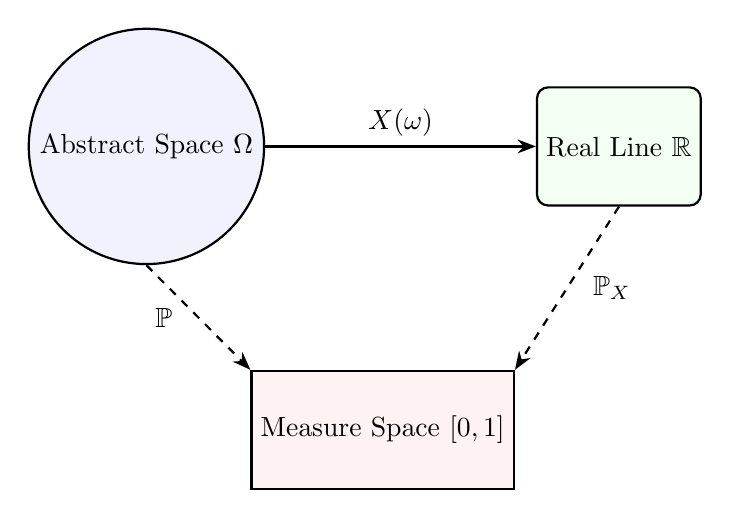
\begin{tikzpicture}[>=Stealth, auto, thick, scale=1.2]
    % Nodes
    \node (Omega) at (0, 0) [circle, draw, minimum size=2.5cm, fill=blue!5] {Abstract Space $\Omega$};
    \node (R) at (5, 0) [rectangle, draw, rounded corners, minimum size=1.5cm, fill=green!5] {Real Line $\mathbb{R}$};
    \node (P) at (2.5, -3) [rectangle, draw, minimum size=1.5cm, fill=red!5] {Measure Space $[0, 1]$};
    
    % Arrows
    \draw[->] (Omega.east) -- node[above] {$X(\omega)$} (R.west);
    \draw[->, dashed] (Omega.south) -- node[left, xshift=-2mm] {$\mathbb{P}$} (P.north west);
    \draw[->, dashed] (R.south) -- node[right, xshift=2mm] {$\mathbb{P}_X$} (P.north east);
\end{tikzpicture}
\end{center}
\vspace{2mm}

\subsection{Heuristics, "Cheats", and Fallacies}
\begin{itemize}
    \item \textbf{Heuristic:} If a problem asks for ``at least one'' or ``at most one'', immediately compute the complement (e.g., ``none'' or ``all'') as it usually consists of exactly one sample point.
    \item \textbf{Fallacy (The Equiprobability Trap):} Assuming that because there are $N$ outcomes, each has probability $1/N$ (seen in Problem 2.25). Always verify if the physical generative process is uniformly random.
    \item \textbf{Fallacy (Confusing Disjoint with Independent):} Two events are disjoint (mutually exclusive) if $A \cap B = \emptyset$. They are independent if $\mathbb{P}(A \cap B) = \mathbb{P}(A)\mathbb{P}(B)$. Disjoint events are actually \textit{maximally dependent} (if one happens, the other definitively cannot).
\end{itemize}

% ==========================================
% PART 5
% ==========================================
\section{Part 5: Conceptual Synthesis and The "Big Picture"}

\subsection{A) Thematic Connections}
The central unifying theme of this chapter is the transition from **Qualitative Logic to Quantitative Measure**. Set theory allows us to qualitatively describe relationships between events (unions, intersections, subsets). Kolmogorov's genius was defining a mathematical operator (the measure $\mathbb{P}$) that acts as a bridge, preserving the algebra of sets while assigning a continuous numerical weight (from 0 to 1) to those sets. This establishes a structural isomorphism between Boolean logical operations and arithmetic addition/subtraction.

\subsection{B) Forward and Backward Links}
\begin{itemize}
    \item \textbf{Backward Links:} This builds entirely on Naive Set Theory (Cantor) and basic combinatorics (Euler/Pascal). 
    \item \textbf{Forward Links:} This sets the absolute bedrock for Measure Theory and Lebesgue Integration. Understanding that probability operates on subsets (Events) rather than individual points is crucial for advanced Statistics and Stochastic Calculus. Later, continuous distributions will force us to abandon the power set $\mathcal{P}(\Omega)$ and use \textit{Borel $\sigma$-algebras} to avoid paradoxes of non-measurable sets (like the Banach-Tarski paradox).
\end{itemize}

% ==========================================
% PART 6
% ==========================================
\section{Part 6: Abstract Real-World Modeling (AI, ML, \& Quant Finance)}

\subsection{A) Concrete Scenarios}
\begin{enumerate}
    \item \textbf{Algorithmic Trading (Quantitative Finance):} High-frequency trading models rely on updating the probability of asset price movements based on incoming order book data. This relies heavily on conditional probability and filtrations (a sequence of expanding event spaces).
    \item \textbf{Bayesian Neural Networks (AI):} Unlike standard deterministic neural nets, Bayesian nets treat the weights of the network as random variables defined over a probability space, allowing the AI to quantify its own epistemic uncertainty.
\end{enumerate}

\subsection{B) Model Problem Setup: Stochastic Calculus \& Option Pricing}
In advanced Quantitative Finance, the simple discrete sample space $S$ is replaced by the space of continuous functions $\Omega = C([0,T], \mathbb{R})$, representing all possible continuous price paths of an asset.
\newline\newline
\textbf{The Theoretical Framework:}
Let $(\Omega, \mathcal{F}, \mathbb{P})$ be our probability space, equipped with a \textit{filtration} $\{\mathcal{F}_t\}_{t \ge 0}$, representing the information available in the market up to time $t$. The asset price $S_t$ is a stochastic process modeled by the Geometric Brownian Motion (GBM) Stochastic Differential Equation (using Ito's Calculus):
\[ dS_t = \mu S_t dt + \sigma S_t dW_t \]
where $W_t$ is a standard Wiener process (Brownian motion) under the real-world measure $\mathbb{P}$. 

To price a European Call Option with payoff $C_T = \max(S_T - K, 0)$, we cannot simply take the expected value under $\mathbb{P}$. We must use Girsanov's Theorem to find an equivalent \textit{risk-neutral measure} $\mathbb{Q}$ such that the discounted asset price $e^{-rt}S_t$ is a martingale (fair game). The price of the option is thus the rigorously defined Lebesgue integral:
\[ C_0 = e^{-rT} \mathbb{E}^{\mathbb{Q}}[ \max(S_T - K, 0) ] = e^{-rT} \int_{\Omega} \max(S_T(\omega) - K, 0) \, d\mathbb{Q}(\omega) \]
This model, which won the Nobel Prize (Black-Scholes-Merton), is purely an application of the fundamental axioms of probability spaces extrapolated to continuous time.

% ==========================================
% PART 7
% ==========================================
\section{Part 7: Common Variations and Untested Concepts}

The homework provided focuses entirely on finite, discrete sample spaces. A critical concept not tested is the \textbf{Continuity of Probability Measure}, which bridges finite additivity (Axiom 3 for finite limits) to limits of infinite sequences of sets.

\begin{definition}[$\sigma$-algebra]
To handle uncountable spaces (like the real line $\mathbb{R}$), the event space $\mathcal{F}$ must be a $\sigma$-algebra:
1) $\Omega \in \mathcal{F}$ \quad 2) If $A \in \mathcal{F}$, then $\overline{A} \in \mathcal{F}$ \quad 3) If $A_1, A_2, \dots \in \mathcal{F}$, then $\bigcup_{i=1}^\infty A_i \in \mathcal{F}$.
\end{definition}

\begin{theorem}[Continuity of Measure from Below]
If $A_1 \subset A_2 \subset A_3 \subset \dots$ is an increasing sequence of events in $\mathcal{F}$, let $A = \bigcup_{i=1}^\infty A_i$. Then $\lim_{n \to \infty} \mathbb{P}(A_n) = \mathbb{P}(A)$.
\end{theorem}
\begin{proof}[Rigorous Proof]
We define a new sequence of disjoint sets: let $B_1 = A_1$, and for $n \ge 2$, let $B_n = A_n \cap \overline{A_{n-1}}$. 
The sets $\{B_n\}$ are mutually exclusive, and by construction, $\bigcup_{i=1}^n B_i = A_n$, and $\bigcup_{i=1}^\infty B_i = A$.
By Axiom 3 (Countable Additivity):
\[ \mathbb{P}(A) = \mathbb{P}\left(\bigcup_{i=1}^\infty B_i\right) = \sum_{i=1}^\infty \mathbb{P}(B_i) = \lim_{n \to \infty} \sum_{i=1}^n \mathbb{P}(B_i) \]
Since $\sum_{i=1}^n \mathbb{P}(B_i) = \mathbb{P}\left(\bigcup_{i=1}^n B_i\right) = \mathbb{P}(A_n)$, it follows that $\mathbb{P}(A) = \lim_{n \to \infty} \mathbb{P}(A_n)$.
\end{proof}

% ==========================================
% PART 8
% ==========================================
\section{Part 8: Advanced Diagnostic Testing: "Find the Flaw"}

Below are five mathematical proofs regarding set theory and probability. Each contains a subtle, critical logical flaw. Your task as the grader is to identify the error. (Solutions are at the bottom).

\prob{Flaw 1} \textbf{Theorem:} Mutually exclusive events are independent.
\newline \textbf{Proof:} Let $A$ and $B$ be mutually exclusive events. By the addition rule, $\mathbb{P}(A \cup B) = \mathbb{P}(A) + \mathbb{P}(B) - \mathbb{P}(A \cap B)$. Because they are mutually exclusive, Axiom 3 dictates $\mathbb{P}(A \cup B) = \mathbb{P}(A) + \mathbb{P}(B)$. Equating the two yields $\mathbb{P}(A \cap B) = 0$. Since the probability of their intersection is 0, they do not overlap, meaning the occurrence of one does not affect the other. Therefore, they are independent. \qedsymbolcustom

\prob{Flaw 2} \textbf{Theorem:} On an infinite discrete space, all outcomes can be equally likely.
\newline \textbf{Proof:} Consider the sample space of all natural numbers $\Omega = \mathbb{N}$. Let the probability of choosing any specific number $n$ be $\mathbb{P}(n) = \epsilon$. Assume $\epsilon > 0$. By countable additivity, $\mathbb{P}(\Omega) = \sum_{n=1}^\infty \epsilon = \infty$, which violates Axiom 2. Therefore, we must set $\epsilon = 0$. Then $\mathbb{P}(\Omega) = \sum_{n=1}^\infty 0 = 0$. Since $\mathbb{P}(\Omega)$ must equal 1, $1=0$. This is a paradox showing that math breaks down at infinity. \qedsymbolcustom

\prob{Flaw 3} \textbf{Theorem:} The probability of getting at least one Head in two coin flips is $2/3$.
\newline \textbf{Proof:} When flipping two balanced coins, we can count the total number of heads. The possible outcomes for the total number of heads are $S = \{0, 1, 2\}$. The event ``at least one head'' corresponds to the subset $A = \{1, 2\}$. Since $A$ contains 2 out of the 3 possible outcomes in the sample space, $\mathbb{P}(A) = 2/3$. \qedsymbolcustom

\prob{Flaw 4} \textbf{Theorem:} The sets $A \cap (B \cup C)$ and $(A \cap B) \cup C$ are logically equivalent.
\newline \textbf{Proof:} We will use Venn diagram logic. Suppose $x \in A \cap (B \cup C)$. This means $x$ is in $A$, and $x$ is in either $B$ or $C$. If $x$ is in $B$, then $x \in A \cap B$, meaning it is in $(A \cap B) \cup C$. If $x$ is in $C$, then it is trivially in $(A \cap B) \cup C$. Since every element maps perfectly, the sets are identical. \qedsymbolcustom

\prob{Flaw 5} \textbf{Theorem:} $\mathbb{P}(A \mid B) + \mathbb{P}(A \mid \overline{B}) = 1$.
\newline \textbf{Proof:} By the Law of Total Probability, $\mathbb{P}(A) = \mathbb{P}(A \cap B) + \mathbb{P}(A \cap \overline{B})$. Dividing the entire equation by $\mathbb{P}(A)$ yields $1 = \mathbb{P}(B \mid A) + \mathbb{P}(\overline{B} \mid A)$. Since the logical conditions are symmetric and arbitrary, we can swap the condition and the event, yielding $\mathbb{P}(A \mid B) + \mathbb{P}(A \mid \overline{B}) = 1$. \qedsymbolcustom

\vspace{1cm}
\subsection*{Solution Key to "Find the Flaw"}
\begin{enumerate}
    \item \textbf{Flaw 1:} The error is the semantic jump from "they do not overlap" to "they do not affect each other". In formal probability, independence requires $\mathbb{P}(A \cap B) = \mathbb{P}(A)\mathbb{P}(B)$. If $\mathbb{P}(A) > 0$ and $\mathbb{P}(B) > 0$, then $\mathbb{P}(A \cap B) = 0 \neq \mathbb{P}(A)\mathbb{P}(B)$. Mutually exclusive events are actually maximally dependent (if $A$ occurs, $B$ is guaranteed not to).
    \item \textbf{Flaw 2:} There is no paradox, the flaw is in the premise. It is a mathematical fact that a uniform probability measure cannot exist on a countably infinite space (like $\mathbb{N}$). You cannot choose an integer "uniformly at random." The proof correctly deduces a contradiction, but incorrectly attributes it to math breaking down rather than concluding the premise (uniform measure on $\mathbb{N}$) is invalid.
    \item \textbf{Flaw 3:} This is the Equiprobability Fallacy (d'Alembert's historical error). The defined sample space $\{0, 1, 2\}$ does not consist of equally likely outcomes. Getting 1 head can happen in two ways ($HT, TH$), while 0 and 2 can only happen one way each. You cannot use the formula $|A|/|S|$ unless the fundamental points are equiprobable.
    \item \textbf{Flaw 4:} The proof shows that $A \cap (B \cup C) \subseteq (A \cap B) \cup C$, but fails to prove the reverse inclusion. If $x \in C$ but $x \notin A$, then $x \in (A \cap B) \cup C$, but $x \notin A \cap (B \cup C)$. Thus, the sets are not equivalent. (The error is assuming one-way implication implies equivalence).
    \item \textbf{Flaw 5:} The error is the assertion "we can swap the condition and the event." Conditional probabilities are not symmetric. The fact that $\mathbb{P}(B \mid A) + \mathbb{P}(\overline{B} \mid A) = 1$ is a valid axiom of probability (fixing the condition space to $A$). Summing across \textit{different} condition spaces ($\mathbb{P}(A \mid B)$ and $\mathbb{P}(A \mid \overline{B})$) has no mathematical constraint and does not sum to 1.
\end{enumerate}

\end{document}